\chapter{まとめと今後の展望}
X線CTは現代医療の画像診断の根幹をなす重要技術であり、年々その検査件数は増加し、適応範囲も拡大している。しかしそれに伴い、医療被ばくに占めるCTの割合が増加傾向にあることが指摘されており、CTの低被ばく化は昨今の医療技術において最重要課題となっている。
本研究では、非常に大きい内部増幅機能をもつ半導体光素子であるMPPCを用いた「低被ばく」かつ「多色」撮影が可能な革新的X線CTシステムを考案し、その最初の実証試験として1mm角のPD,APD,MPPCを用いたCT撮影を実行した。照射X線の線量を変えた際のCT画像を定量評価することで、各検出器で得られた画像の比較を行った。ノイズ・低コントラスト分解能・空間分解能のすべてにおいて、MPPCでは従来型CTのPDによりも同じ線量でも圧倒的に優れた結果が得られ、MPPCを用いることで、低線量下でもPDと同等以上に高い画像S/Nを実現できることが実証できた(3章)。これより被ばく量の問題により使用が制限されてきた子供や妊婦といった患者にも、X線CTによる内部撮影が可能になると期待できる。従来CTの光検出部をMPPCに変えるだけで実現できるため、本研究は早期における臨床応用・実現の点でも非常に優れているといえる。
また、線量自体を1/1,000に下げることができれば、フォトンカウンティングCTの障壁とされてきた高レートの問題を解決することができ、個々のX線パルスについてエネルギーの取得も容易となる(4章)。たとえて言うならば、”白黒テレビがカラーテレビになる” ほど情報量の増加が見込め、様々な多色イメージングが期待される。その一例として、本研究では「コントラストの強調」「ビームハードニングの除去」「K-edgeイメージング」といった多色イメージングを行い、その有用性も検証できた。


\begin{figure}[H]
 \begin{center}
 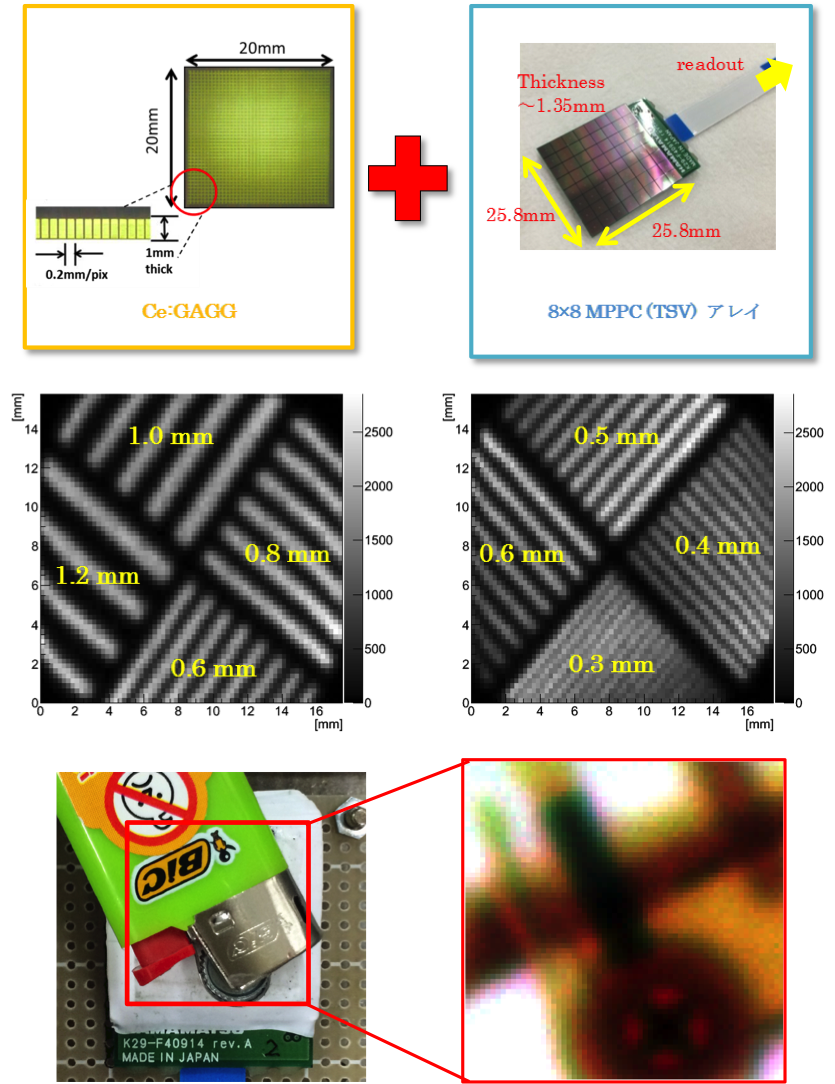
\includegraphics[bb=0.000000 0.000000 400.766870 520.276990,width=1\hsize]{image2/chapter5/oshimaetal.png} 
 \end{center}
 \caption{高精細シンチレータ(GAGG)とMPPCの外観とイメージング結果}
 \label{fig:oshimaetal}
\end{figure}

本研究は、もっとも単純な光センサー単素子による原理実証に重点を置いたが、今後はより実際のCTシステムに近い複合システムへの拡張を考えている。たとえば、MPPCを2次元にアレイ化し、我々がこれまで開発した高精細シンチレータと組み合わせた「多色マルチスライスX線モジュール」の開発を考えている。これまで、YAPシンチレータ同様にフォトンカウンティングに有効なCe;GAGG シンチレータのプレートに0.25-mm ピッチでダイシング加工を施し、8×8 MPPCアレイと組み合わせることで0.3 mmの空間分解能を実現している。また、わずか4chの出力信号を用いて31, 60, 88キロ電子ボルトのX線を用いた「3色イメージング」にも成功した(図4.5; Oshima et al. 2015)。この高精細シンチレータとMPPCアレイを組み合わせ、CTモジュールを作成することで「多色」かつ「低線量」のマルチスライスCTへと発展が可能である。このような高精細シンチレータを用いた低被ばくCTは、簡便かつ低コスト、また既存のCTの置き換えも容易であり、今後ブレークスルーを起こすことも期待できる。現在は怪我をしたときや健康診断の画像診断の入り口はレントゲンなどの一般撮影であるが、一般撮影レベルの被ばく量でCT撮影が可能となればCTも検査の入口として手軽に撮影することが可能になり、病気の早期発見につながる。このように「低被ばく」と「多色化」が切り拓く新たな画像診断の可能性は無限である。本研究が全世界のCTメーカーにCTの変革の可能性を示唆し、新たなCT画像診断の可能性を切り拓く、一石となることを願っている。